
\subsection{Applications}
\label{architecture_s}  


The overall objective is to allow a client to trust a code produced by an untrusted code producer. Our approach is especially suitable
 in cases where the client policy involves non trivial functional or safety requirements and thus, a full automatization of the verification 
process is impossible. To this end, we propose a PCC technique that exploits the JML compiler and the weakest predicate function presented in the article. 
 
 The framework is presented in Fig.~\ref{architecture}; note that certificates and their checking are not yet implemented
 and thus are in oblique font.
  


 \begin{figure}[!tbp]
 \centering
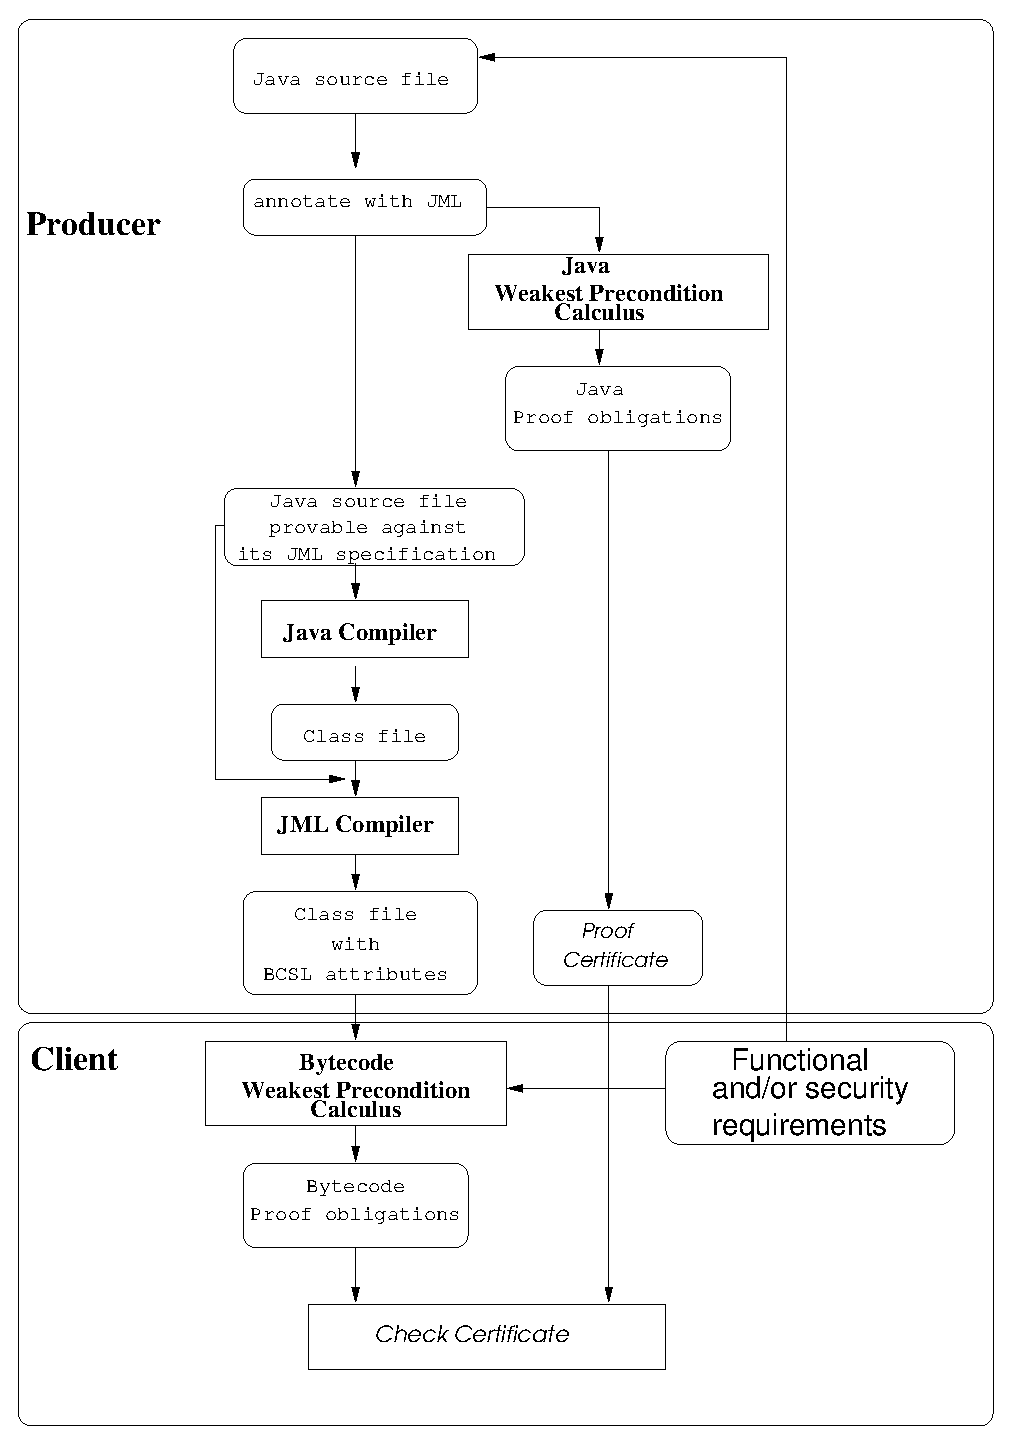
\epsfig{ file=sac/architecture.eps, width=6in, height=6in }
\caption{\sc The overall architecture for client producer scenarios }
\label{architecture}
\end{figure}

In the first stage of the process the client provides the functional
and (or) security requirements to the producer.  The requirements can
be in different form:
\begin{itemize}
\item Typical functional requirements can be a specified interface
describing the application to be developed. In that case, the client
specifies in JML the features that have to be implemented by the code
producer.
\item Client security requirements can be a restricted access to some
method from the API expressed as a finite state machine.  For example,
suppose that the client API provides transaction management facilities
- the API method \texttt{open} for opening and method \texttt{close}
for closing transactions. In this case, a requirement can be for no
nested transactions.  This means that the methods \texttt{open} and
\texttt{close} can be annotated to ensure that the method
\texttt{close} should not be called if there is no transaction running
and the method \texttt{open} should not be called if there is already
a running transaction. In this scenario, we can apply results of
previous work \cite{m+04:cardis}.  
\end{itemize}
Usually, the development process involves annotating the source code
with JML specification, generating verification conditions, using
proof obligation generator over the source code and discharging proofs
which represent the program safety certificate and finally, the
producer sends the certificate to the client along with the annotated
class files.  Yielding certificates over the source code is based on
the observation that proof obligations on the source code and
non-optimized bytecode respectively are syntactically the same modulo
names and basic types. Every Java file of the untrusted code is
normally compiled with a Java compiler to obtain a class file. Every
class file is extended with user defined attributes that contain the
BML specification, resulting from the compilation of the JML
specification of the corresponding Java source file.


We have extended the Jack tool with a compiler from
 JML to BML and a bytecode verification condition generator. In the next sections, we introduce
 the BML language, the JML compiler and the bytecode \wpi calculus which underlines the bytecode verification condition generator.
 
